\chapter{Geometria Analitica}

\section{Retta nel piano}

\subsection{Equazione della retta}

Supponiamo di avere un vettore $v = (l,m)$ non nullo e un punto $P_0 = (x_0,y_0)$ del piano. Vogliamo determinare tutti i punti $P$ appartententi alla retta $r$, passante per il punto $P_0$ e parallela al vettore $v$.

\begin{figure}[H]
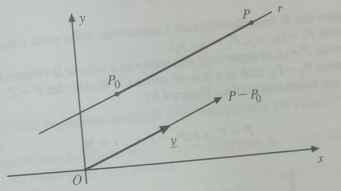
\includegraphics{equazione-retta}
\centering
\end{figure}

Ovviamente il punto $P$ che cerchiamo (generalizzando al caso specifico di un punto solo) appartiene alla retta $r$ se e solo se il vettore $P-P_0$ è parallelo al vettore $\vec{v}$, cioè se esiste una $t$ tale che $P-P_0=t\vec{v}$.

Visto che $P=(x,y)$ e $P_0=(x_0,y_0)$ e $v = (l,m)$ possiamo scrivere
$$
\begin{cases}
x = x_0 + lt \\
y = y_0 + mt
\end{cases}
$$
che è l'equazione parametrica della retta $r$ passante per il punto $P_0$ e parallela al vettore $\vec{v}$.

\subsection{Retta tra due punti}

Supponiamo di voler determinare l'equazione della retta $r$ passante per due punti distinti $P_1=(x_1,y_1)$, $P_2=(x_2,y_2)$.

Un punto $P=(x,y)$ appartiene a $r$ se e solo se il vettore $P-P_1$ è parallelo al vettore $P_2-P_1$. Cioè solo se esiste $t \in \R$ tale che $P-P_1=t(P_2-P_1)$. Da questo otteniamo $$P = P_1+t(P_2-P_1)$$
Sostituendo le coordinate di $P_1$, $P_2$ e $P$ nell'espressione precedente della retta $r$ si ottiene la seguente

$$
r=
\begin{cases}
x = x_1 + t(x_2-x_1) \\
y = y_1 + t(y_2-y_1)
\end{cases}
$$

Al variare di $t$ si ottengono tutti i punti della retta $r$ passante per $P_1,P_2$.

Al variare di $t \in [0,1]$ si ottengono tutti i punti della retta $r$ passante appartenenti al segmento $P_1P_2$.

È possibile ricavare $t$ in questo modo:
$$ t = \frac{x-x_1}{x_2-x_1} = \frac{y-y_1}{y_2-y_1}$$


\begin{definition}
L'equzione normale della retta passante per $P_1,P_2$ è: $$\frac{x-x_1}{x_2-x_1} = \frac{y-y_1}{y_2-y_1}$$
\end{definition}

Se $x_2 - x_1=0$ o $y_2 - y_1=0$ allora l'equazione diventa
$$x-x_1 = 0 \text{ se } x_2 = x_1$$
$$y-y_1 = 0 \text{ se } y_2 = y_1$$

\subsection{Equazione Cartesiana}

\subsubsection{Per due punti}

Dall'equazione normale si ottiene che
$$(x-x_1)(y_2-y_1) = (y-y_1)(x_2-x_1)$$
cioè
$$x(y_2-y_1)-y(x_2-x_1)+y_1x_2-y_2x_1=0$$


\subsubsection{Perpendicolare ad un vettore}

Vogliamo trovare l'equazione della retta $r$ passante per $P_0$ e perpendicolare al vettore $n=(a,b)$.

Cioè se $(P-P_0) \circ n = 0$.

cioè $$a(x-x_0)+b(y-y_0) = 0$$

\subsection{Parallelismo tra rette}

Date due rette $r$ e $r_1$ di equazioni $ax+by+c=0$ e $a_1x+b_1y+c_1=0$, esse sono parallele se e solo se i vettori $n  = (a,b)$ e $n_1 = (a_1,b_1)$, direttori delle rette, sono paralleli, cioè se eiste un $k$ tale per cui $kn = n_1$.


\subsection{Perpendicolarità tra rette}

Date due rette $r$ e $r_1$ di equazioni $ax+by+c=0$ e $a_1x+b_1y+c_1=0$, esse sono parallele se e solo se il prodotto scalare dei vettori $n  = (a,b)$ e $n_1 = (a_1,b_1)$, direttori delle rette, è nullo.

$$aa_1+bb_1 = 0$$

\subsection{Angolo tra due rette}

Date

$$
r = \begin{cases}
x = x_0 + lt \\
y = y_0 + mt
\end{cases}
$$

$$
r_1 = \begin{cases}
x = x_1 + l_1t \\
y = y_1 + m_1t
\end{cases}
$$

l'angolo tra le rette $r,r_1$ è uguale all'angolo tra i vettori $v_r$ e $v_{r_1}$, cioè

$$\arccos(\pm (v_r \circ v_{r_1}))$$

\subsection{Equazione in forma esplicita}

Sia data la retta $r$ di equazione $ax+by+c=0$. Supponiamo $b \neq 0$, allora
$$y = -\frac{a}{b} x - \frac{c}{b}$$
Ponendo $m= -\frac{a}{b}$ e $q = -\frac{c}{b}$ si ottiene $y=mx+q$.

Questa formula fornisce l'equazione di tutte le rette del piano, eccetto le rette $x=k$, parallele all'asse $y$.

$m$ è detto il coefficiente angolare della reta.

Ponendo $x=t$

$$
\begin{cases}
x= t \\
y=q+mt
\end{cases}
$$

Inoltre
$m = \tan(\theta)$


\subsection{Distanza punto - retta}

Siano dati nel piano una retta $r$ di equazione $ax+by+c=0$ e un punto $P = (x_0,y_0)$.

Sia $H$ il piede della perpendicolare lla retta $r$ condotta da $P_0$.

La misura del segmento $P_0H$ ovvero il numero $\gamma = ||P_0-H||$ è la distanza del punto $P_0$ dalla retta $r$.

Poichè $H \in r$ allora $ax_H+by_h+c=0$.

$P_0-H$ è un vettore parallelo a $v=(a,b)$ (perpendicolare alla retta $r$), quindi $$|(P_0-H) \circ v| = ||(P_0-H)|| \cdot ||v||$$

cioè

$$\gamma = ||P_0-H|| = \frac{|(P_0-H)\circ \vec{v}|}{||\vec{v}||}$$

che alla fine è

$$\gamma = \frac{|ax+by_0+c|}{\sqrt{a^2+b^2}}$$

\subsubsection{Distanza rette parallele}

$$\gamma = \frac{|-c_1 + c|}{\sqrt{a^2+b^2}}$$

\section{Retta nello spazio}

\subsection{Equazione parametrica}

Siano dati un punto $P_0$ nello spazio e un vettore non nullo $v$. Un punto $P$ appartiene alla retta $r$ passante per $P_0$ e parallela a $v$ se e solo se il vettore $P-P_0$ è parallelo al vettore $v$, ossia se e solo se esiste $t \in \R$ tale che $$P-P_0=tv$$

$$
\begin{cases}
x = x_0 + lt \\
y = y_0 + mt \\
z = z_0 + nt
\end{cases}
$$

\subsection{Retta tra due punti}

Si ragiona in modo analogo a quanto fatto nel piano, considerando chiaramente un punto in più.

\section{Piano}

\begin{figure}[H]
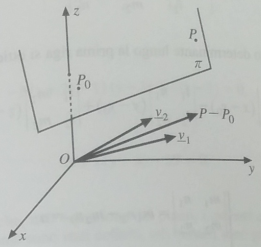
\includegraphics{piano}
\centering
\end{figure}

Dato un punto $P_0$ e due vettori non paralleli dello spazio $v_1=l_1i+m_1j+n_1k$ e $v_2=l_2i+m_2j+n_2k$

Un punto $P$ appartiene al piano  $\pi$ passante per $P_0$ e parallelo ai vettori $v_1$ e $v_2$ se e sole se il vettore $P-P_0$ è complanare con i vettori $v_1$ e $v_2$ ovvero se e solo se esistono $\alpha, \beta \in \R$ tali che $$P-P_0 = \alpha v_1 + \beta v_2$$

Da qui otteniamo l'equazione parametrica del piano

$$
\begin{cases}
x = x_0 + \alpha l_1 + \beta l_2 \\
y = y_0 + \alpha m_1 + \beta m_2 \\
z = z_0 + \alpha n_1 + \beta n_2
\end{cases}
$$

\subsection{Appartenenza al piano}

Consideriamo la seguente matrice

$$
\begin{matrix}
x-x_0 & y-y_0 & z-z_0 \\
l_1 & m_1 & n_1 \\
l_2 & m_2 & n_2
\end{matrix}
$$

La prima riga è combinazione lineare delle altre due, quindi il determinante è uguale a zero.

Un punto $P$ appartiene al piano se e solo se il determinante della matrice è uguale a 0.

Cioè

$$
\begin{vmatrix}
m_1 & n_1 \\
m_2 & n_2 \\
\end{vmatrix}
(x-x_0)
-
\begin{vmatrix}
l_1 & n_1 \\
l_2 & n_2 \\
\end{vmatrix}
(y-y_0)
+
\begin{vmatrix}
l_1 & m_1 \\
l_2 & m_2 \\
\end{vmatrix}
(z-z_0) = 0
$$

Ponendo

$$
\begin{cases}
\begin{vmatrix}
m_1 & n_1 \\
m_2 & n_2 \\
\end{vmatrix} = a \\
- \begin{vmatrix}
l_1 & n_1 \\
l_2 & n_2 \\
\end{vmatrix} = b \\
\begin{vmatrix}
l_1 & m_1 \\
l_2 & m_2 \\
\end{vmatrix} = c
\end{cases}
$$

si ottiene l'equazione di tutti i piani passanti per $P_0$.
$$
a(x-x_0) + b(y-y_0) + c(z-z_0) = 0
$$

\subsection{Equazione piano alternativa}

Siano dati un punto $P_0$ dello spazio e un vettore $u$.

Un punto $P$ appartiene al piano passante per $P_0$ e perpendicolare a $u$ se e solo se il vettore $P-P_0$ è perpendicolare a $u$, cioè $$(P-P_0) \circ u =0$$

Poiché $P-P_0 = (x-x_0)i + (y-y_0)j +(z-z_0)k$ allora $$ a(x-x_0) + b(y-y_0) +c(z-z_0) = 0$$

\subsection{Piano per tre punti}

Se
$$
\begin{vmatrix}
P_{generico} - P_1
P_2 - P_1
p_3 - P_1
\end{vmatrix} = 0
$$

\subsection{Parallelismo e perpendicolarità tra piani}

Due piani sono paralleli se e solo se i vettori $u$ $u_1$, perpendicolari al piano, sono paralleli, cioè se e solo se esiste $k \in \R$ tale che $$u = k u_1$$

\subsection{Perpendicolarità tra piani}

Due piani sono paralleli se e solo se i vettori $u$ $u_1$, perpendicolari al piano, sono paralleli, cioè se e solo se il loro prodotto scalare è 0.

\subsection{Intersezione di due piani}

Quando due piani si intersecano danno origine ad una retta.

$$
r =
\begin{cases}
a_1x+b_1y+c_1z+d_1 = 0 \\
a_2x+b_2y+c_2z+d_2 = 0 \\
\end{cases}
$$

\subsection{Fasci di piani}

Esisono infiniti piani che passano per una retta $r$. L'insieme di tutti questi piani si chiama fascio di piani di asse $r$.

Se

$$
r =
\begin{cases}
a_1x+b_1y+c_1z+d_1 = 0 \\
a_2x+b_2y+c_2z+d_2 = 0 \\
\end{cases}
$$

allora il fascio di piani individuato è dato da

$$
\lambda(a_1x+b_1y+c_1z+d_1) + \mu (a_2x+b_2y+c_2z+d_2) = 0
$$


\subsection{Parallelismo e perpendicolarità tra una retta e un piano}

\subsubsection{Parallelismo}

\begin{figure}[H]
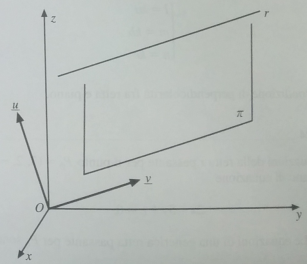
\includegraphics{parallelismo-piano-retta}
\centering
\end{figure}

Il prodotto scalare dei due vettori direttori deve essere 0.

\subsubsection{Perpendicolarità}

\begin{figure}[H]
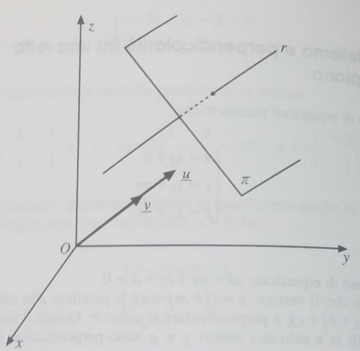
\includegraphics{perpendicolarita-piano-retta}
\centering
\end{figure}

I due vettori direttori devono essere proporzionali.


\subsection{Angolo tra due piani}

È l'angolo tra i due vettori direttori normali ai due piani.

$$\cos(\alpha) = \frac{|a \circ b|}{||a|| \cdot ||b||}$$

\subsection{Angolo tra una retta e un piano}

\begin{figure}[H]
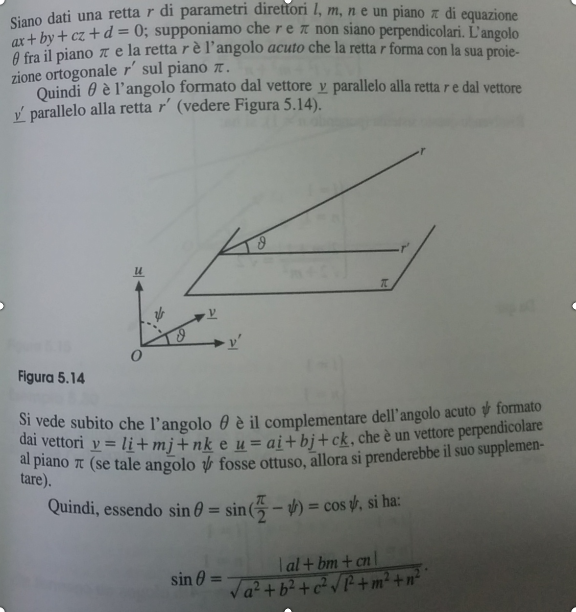
\includegraphics{angolo-retta-piano7}
\centering
\end{figure}

\subsection{Rette sghembe}
Due rette si dicono sghembe se non sono complanari, quindi né incidenti né parallele.

Quindi il sistema associato non ha soluzione e i vettori direttori non sono proporzionali.